\chapter{Programación de la HMI}
\label{ap:programacion}
\label{ap:codigo_prueba_ph}

\section*{Máquina de estados de la HMI}

La Figura~\ref{fig:fsm_hmi} muestra la máquina de estados finitos que gobierna
la navegación entre pantallas de la interfaz gráfica. Al arrancar, la
\textit{Pantalla de Carga} verifica el hardware y los simuladores; si detecta
un fallo de sensor transiciona a la \textit{Pantalla de Error}, y si todo es
correcto avanza a la \textit{Pantalla Principal}. Desde ahí el operador puede
iniciar un nuevo proyecto, cargar uno existente, acceder a ajustes o consultar
el registro de experimentos.

\begin{figure}[H]
  \centering
  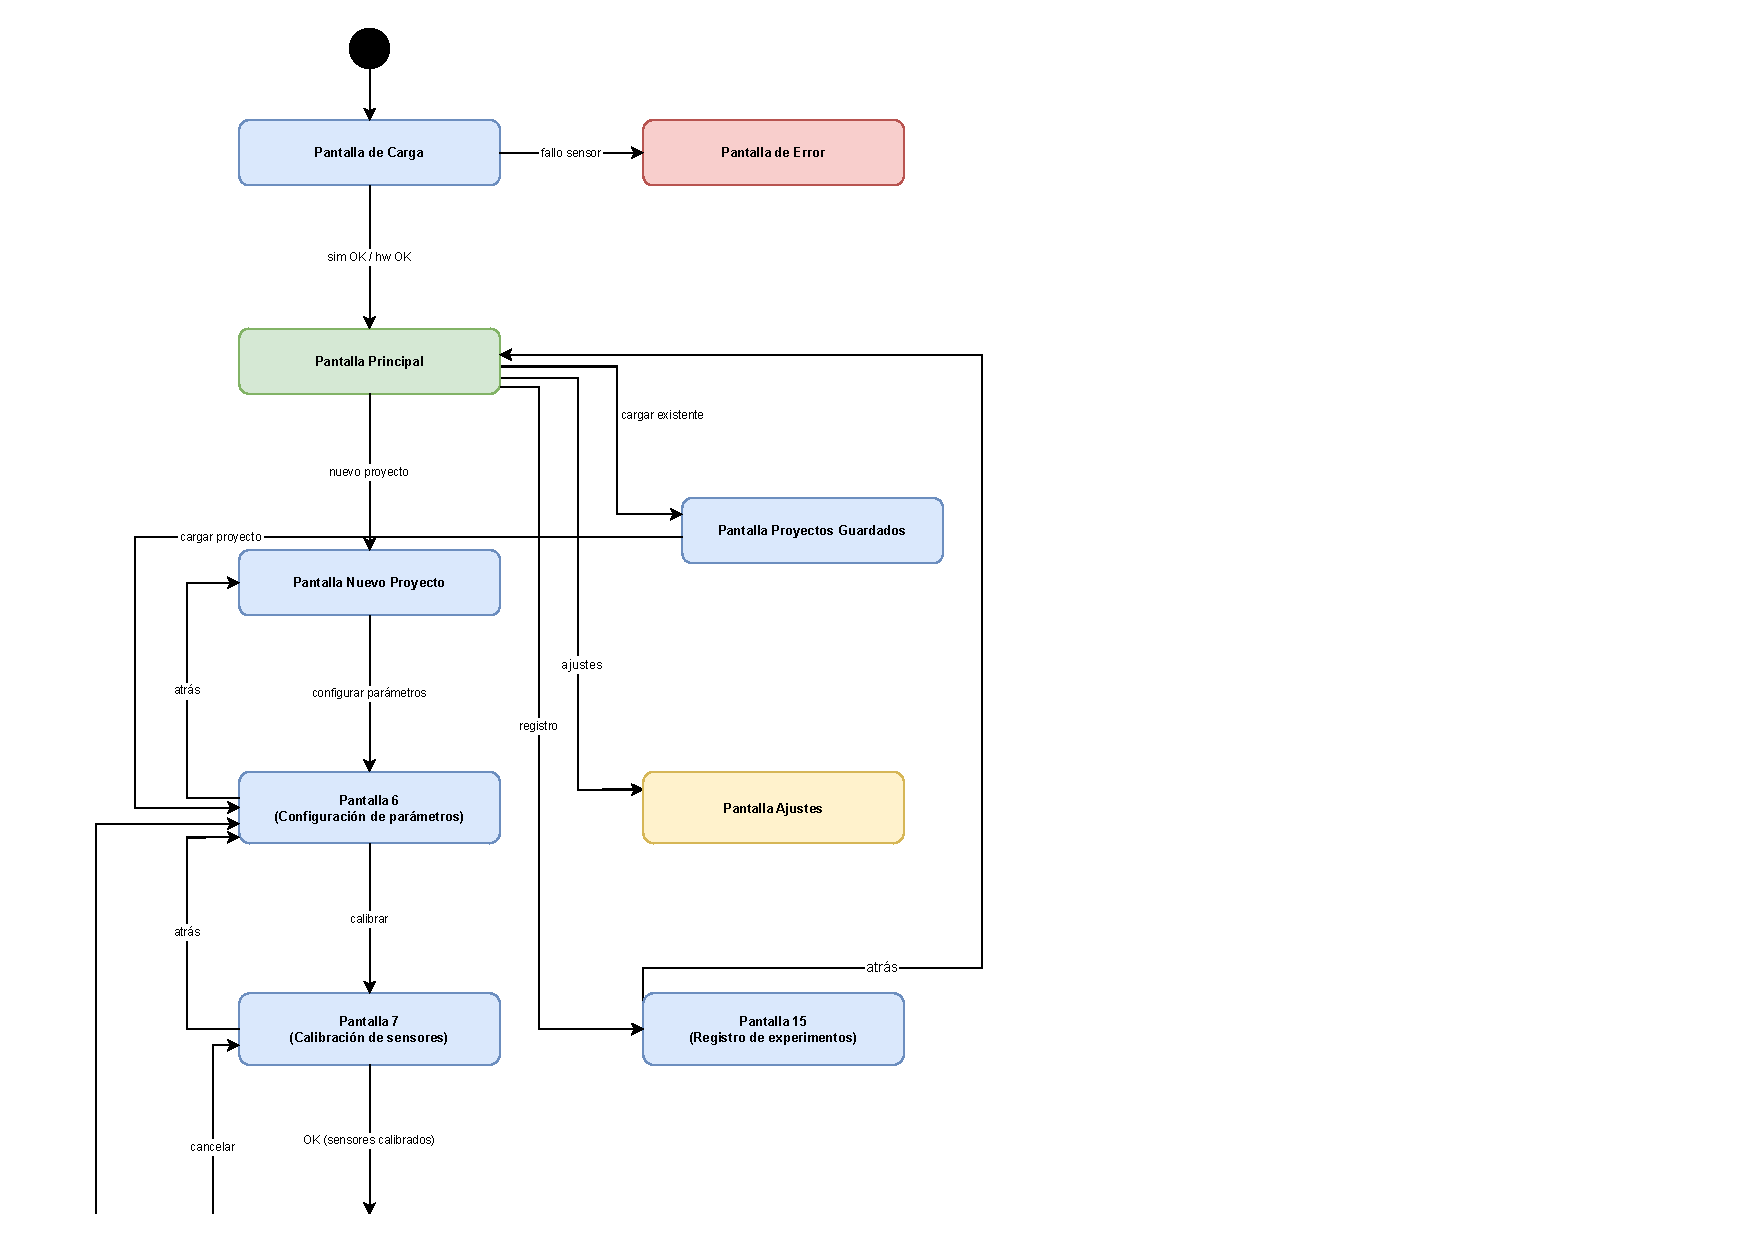
\includegraphics[width=\textwidth]{Figuras/fsm_hmi.pdf}
  \caption{Máquina de estados finitos de la HMI del biorreactor. Los nodos
           representan pantallas y las aristas las transiciones disparadas por
           eventos de usuario o del sistema.}
  \label{fig:fsm_hmi}
\end{figure}

\section*{Mockups de la interfaz HMI}

\begin{figure}[H]
  \centering
  
\includegraphics[width=0.75\textwidth]{mockup_1}
  \caption{Mockup A1 --- Pantalla de inicio.}
  \label{fig:mockup_a1}
\end{figure}

\begin{figure}[H]
  \centering
  
\includegraphics[width=0.75\textwidth]{mockup_2}
  \caption{Mockup A2/A33 --- Error de carga del sistema.}
  \label{fig:mockup_a2a33}
\end{figure}

\begin{figure}[H]
  \centering
  
\includegraphics[width=0.75\textwidth]{mockup_3}
  \caption{Mockup A3 --- Menú principal.}
  \label{fig:mockup_a3}
\end{figure}

\begin{figure}[H]
  \centering
  
\includegraphics[width=0.75\textwidth]{mockup_4}
  \caption{Mockup A4 --- Gestión de proyectos.}
  \label{fig:mockup_a4}
\end{figure}

\begin{figure}[H]
  \centering
  
\includegraphics[width=0.75\textwidth]{mockup_5}
  \caption{Mockup A5 --- Configuración de parámetros.}
  \label{fig:mockup_a5}
\end{figure}

\begin{figure}[H]
  \centering
  
\includegraphics[width=0.75\textwidth]{mockup_6}
  \caption{Mockup A6 --- Teclado de entrada.}
  \label{fig:mockup_a6}
\end{figure}

\begin{figure}[H]
  \centering
  
\includegraphics[width=0.75\textwidth]{mockup_7}
  \caption{Mockup A7 --- Nombrar proyecto.}
  \label{fig:mockup_a7}
\end{figure}

\begin{figure}[H]
  \centering
  
\includegraphics[width=0.75\textwidth]{mockup_8}
  \caption{Mockup A8 --- Confirmación de datos.}
  \label{fig:mockup_a8}
\end{figure}

\begin{figure}[H]
  \centering
  
\includegraphics[width=0.75\textwidth]{mockup_9}
  \caption{Mockup A9 --- Lista de proyectos guardados (pág. 1).}
  \label{fig:mockup_a9}
\end{figure}

\begin{figure}[H]
  \centering
  
\includegraphics[width=0.75\textwidth]{mockup_10}
  \caption{Mockup A10 --- Lista de proyectos guardados (pág. 2).}
  \label{fig:mockup_a10}
\end{figure}

\begin{figure}[H]
  \centering
  
\includegraphics[width=0.75\textwidth]{mockup_11}
  \caption{Mockup A11 --- Información de archivo (lista 1).}
  \label{fig:mockup_a11}
\end{figure}

\begin{figure}[H]
  \centering
  
\includegraphics[width=0.75\textwidth]{mockup_12}
  \caption{Mockup A12 --- Información de archivo (lista 2).}
  \label{fig:mockup_a12}
\end{figure}

\begin{figure}[H]
  \centering
  
\includegraphics[width=0.75\textwidth]{mockup_13}
  \caption{Mockup A13 --- Confirmación de carga (archivo 1).}
  \label{fig:mockup_a13}
\end{figure}

\begin{figure}[H]
  \centering
  
\includegraphics[width=0.75\textwidth]{mockup_14}
  \caption{Mockup A14 --- Confirmación de carga (archivo 2).}
  \label{fig:mockup_a14}
\end{figure}

\begin{figure}[H]
  \centering
  
\includegraphics[width=0.75\textwidth]{mockup_15}
  \caption{Mockup A15 --- Calibración de sensores.}
  \label{fig:mockup_a15}
\end{figure}

\begin{figure}[H]
  \centering
  
\includegraphics[width=0.75\textwidth]{mockup_16}
  \caption{Mockup A16 --- Pantalla de operación principal.}
  \label{fig:mockup_a16}
\end{figure}

\begin{figure}[H]
  \centering
  
\includegraphics[width=0.75\textwidth]{mockup_17}
  \caption{Mockup A17 --- Configuración de tabla de visualización.}
  \label{fig:mockup_a17}
\end{figure}

\begin{figure}[H]
  \centering
  
\includegraphics[width=0.75\textwidth]{mockup_18}
  \caption{Mockup A18 --- Proceso finalizado exitosamente.}
  \label{fig:mockup_a18}
\end{figure}

\begin{figure}[H]
  \centering
  
\includegraphics[width=0.75\textwidth]{mockup_19}
  \caption{Mockup A19 --- Pausa del proceso.}
  \label{fig:mockup_a19}
\end{figure}

\begin{figure}[H]
  \centering
  
\includegraphics[width=0.75\textwidth]{mockup_20}
  \caption{Mockup A20 --- Gestión de proyectos fase 2.}
  \label{fig:mockup_a20}
\end{figure}

\begin{figure}[H]
  \centering
  
\includegraphics[width=0.75\textwidth]{mockup_21}
  \caption{Mockup A21 --- Menú de pausa.}
  \label{fig:mockup_a21}
\end{figure}

\begin{figure}[H]
  \centering
  
\includegraphics[width=0.75\textwidth]{mockup_22}
  \caption{Mockup A22 --- Inicio de vaciado nivel 1.}
  \label{fig:mockup_a22}
\end{figure}

\begin{figure}[H]
  \centering
  
\includegraphics[width=0.75\textwidth]{mockup_23}
  \caption{Mockup A23 --- Confirmación de vaciado nivel 1.}
  \label{fig:mockup_a23}
\end{figure}

\begin{figure}[H]
  \centering
  
\includegraphics[width=0.75\textwidth]{mockup_24}
  \caption{Mockup A24 --- Espera vaciado nivel 1.}
  \label{fig:mockup_a24}
\end{figure}

\begin{figure}[H]
  \centering
  
\includegraphics[width=0.75\textwidth]{mockup_25}
  \caption{Mockup A25 --- Inicio de vaciado nivel 2.}
  \label{fig:mockup_a25}
\end{figure}

\begin{figure}[H]
  \centering
  
\includegraphics[width=0.75\textwidth]{mockup_26}
  \caption{Mockup A26 --- Confirmación de vaciado nivel 2.}
  \label{fig:mockup_a26}
\end{figure}

\begin{figure}[H]
  \centering
  
\includegraphics[width=0.75\textwidth]{mockup_27}
  \caption{Mockup A27 --- Proceso finalizado.}
  \label{fig:mockup_a27}
\end{figure}

\begin{figure}[H]
  \centering
  
\includegraphics[width=0.75\textwidth]{mockup_28}
  \caption{Mockup A28 --- Configuración de guardado.}
  \label{fig:mockup_a28}
\end{figure}

\begin{figure}[H]
  \centering
  
\includegraphics[width=0.75\textwidth]{mockup_29}
  \caption{Mockup A29 --- Nombre del archivo a guardar.}
  \label{fig:mockup_a29}
\end{figure}

\begin{figure}[H]
  \centering
  
\includegraphics[width=0.75\textwidth]{mockup_30}
  \caption{Mockup A30 --- Confirmación de guardado.}
  \label{fig:mockup_a30}
\end{figure}

\begin{figure}[H]
  \centering
  
\includegraphics[width=0.75\textwidth]{mockup_31}
  \caption{Mockup A31 --- Recordatorio de limpieza.}
  \label{fig:mockup_a31}
\end{figure}

\begin{figure}[H]
  \centering
  
\includegraphics[width=0.75\textwidth]{mockup_32}
  \caption{Mockup A32 --- Exportación de datos.}
  \label{fig:mockup_a32}
\end{figure}

\begin{figure}[H]
  \centering
  
\includegraphics[width=0.75\textwidth]{mockup_33}
  \caption{Mockup A34 --- Espera vaciado nivel 2.}
  \label{fig:mockup_a34}
\end{figure}

\begin{figure}[H]
  \centering
  
\includegraphics[width=0.75\textwidth]{mockup_34}
  \caption{Mockup A35 --- Alerta de error en monitoreo.}
  \label{fig:mockup_a35}
\end{figure}

\begin{figure}[H]
  \centering
  
\includegraphics[width=0.75\textwidth]{mockup_35}
  \caption{Mockup Extra --- Pantalla adicional.}
  \label{fig:mockup_extra}
\end{figure}

% ─────────────────────────────────────────────────────────────────────────────
\section*{Interfaz de pruebas del control difuso de pH}

\texttt{prueba\_visual\_ph.py} (v1.2) es la interfaz Tkinter ejecutada en la
Raspberry Pi durante todas las pruebas del sistema de control de pH.
Gestiona la lectura por RS-485 del sensor RK500-12, el control I\textsuperscript{2}C
del PCA9685 (actuadores), la lectura del sensor de nivel XM125 y el lazo de
control difuso SISO de manera concurrente. A continuación se presentan las
tres secciones más relevantes del código.

\begingroup
\lstset{language=Python,
        basicstyle=\ttfamily\scriptsize,
        numbers=left, numberstyle=\tiny,
        frame=single, backgroundcolor=\color{gray!10},
        breaklines=true, breakatwhitespace=true}

\bigskip
\noindent\textbf{1. Constantes de hardware}

\begin{lstlisting}
# Hardware -- constantes
GPIO_OE       = 17
GPIO_ZC       = 27
SERIAL_PORT   = '/dev/ttyAMA0'
SERIAL_BAUD   = 9600
PCA_ADDR      = 0x40
XM125_ADDR    = 0x52
QUERY_PH      = bytes.fromhex('030300000006C42A')

CH_BURBUJEO   = 2    # Bomba de aire / burbujeo
CH_NEUT_A     = 3    # Bomba Neutralizador 1 (en serie)
CH_NEUT_B     = 4    # Bomba Neutralizador 2 (en serie)
CH_TIRA_LED   = 5    # Tira LED
CH_BOMBA_VAC1 = 8    # BombaVaciado 1
CH_BOMBA_VAC2 = 10   # BombaVaciado 2

# Comandos de calibracion Modbus RTU (esclavo 0x03, FC06)
_SLAVE   = 0x03
_CAL_REG = 0x0055   # Registro de calibracion RK500-12
_CAL_VAL = {4: 0x0004, 7: 0x0007, 10: 0x000A}

# Estado del sistema en tiempo de ejecucion
state = {
    'sp': 6.5,  'nivel_max': 100.0, 'nivel_hist': 95.0,
    'ts_s': 30, 'banda': 0.1,  'k_pulso': 2.0,
    'tp_max': 20.0, 'e_max': 0.8,  'e_sat': 0.8,
}
\end{lstlisting}

\bigskip
\noindent\textbf{2. Lógica difusa SISO (idéntica al módulo C++)}

\begin{lstlisting}
def _trimf(x, a, b, c):
    if x <= a or x >= c: return 0.0
    return (x-a)/(b-a) if x <= b else (c-x)/(c-b)

def _trapmf(x, a, b, c, d):
    if x <= a or x >= d: return 0.0
    if b <= x <= c: return 1.0
    return (x-a)/(b-a) if x < b else (d-x)/(d-c)

MFS_E = {
    # Rango de control fino: [0, 0.8] pH
    'N':  ([0.0,  0.0,  0.06],       _trimf ),  # nulo
    'PE': ([0.04, 0.15, 0.28],       _trimf ),  # pequenio
    'ME': ([0.22, 0.35, 0.50],       _trimf ),  # mediano
    'GE': ([0.42, 0.58, 0.75],       _trimf ),  # grande
    'MG': ([0.65, 0.80, 0.80, 0.80], _trapmf),  # muy grande -> maximo
}
MFS_S = {
    'OFF':   ([0.0, 0.0,  1.5],          _trimf ),  # zona muerta
    'POCO':  ([3.0, 5.0,  7.0],          _trimf ),  # centro 5 s -> 10 s efectivo
    'MEDIO': ([5.5, 7.0,  9.0],          _trimf ),  # centro 7 s -> 14 s efectivo
    'MUCHO': ([7.5, 9.0, 10.0],          _trimf ),  # centro 9 s -> 18 s efectivo
    'MAX':   ([9.5, 10.0, 10.0, 10.0],   _trapmf),  # 10 s -> 20 s efectivo
}
REGLAS = [('N','OFF'),('PE','POCO'),('ME','MEDIO'),('GE','MUCHO'),('MG','MAX')]

def fuzzy(error, e_max=None):
    """Inferencia Mamdani + defusificacion CoG. Retorna t_int en [0, 10] s."""
    if e_max is None: e_max = E_MAX
    e = max(0.0, min(e_max, error))   # recorte al universo de control
    num = den = 0.0
    for i in range(71):               # 71 puntos uniformes en [0, 10]
        x  = i * 10.0 / 70
        mu = max(min(fn(e, *p), fn2(x, *p2))
                 for (en, sn) in REGLAS
                 for p, fn  in [MFS_E[en]]
                 for p2, fn2 in [MFS_S[sn]])
        num += x * mu; den += mu
    return num / den if den > 0 else 0.0
\end{lstlisting}

\bigskip
\noindent\textbf{3. Lazo de control --- toma de decisión por ciclo}

Cada $T_s = 30$~s el hilo de control evalúa el error de pH y decide el
tiempo de pulso: prefiltro de banda muerta, saturación directa si
$e \geq e_\text{sat} = 0.8$~pH, o inferencia difusa para errores intermedios.
El resultado se escala por $k_\text{pulso} = 2$ antes de activar la bomba (CH3+CH4).

\begin{lstlisting}
# --- Evaluacion cada Ts (configurable desde GUI) ---
error = sp - ph
with _lock: state['error'] = error

with _lock: banda = state['banda']
nivel_ok = (nivel is None) or (nivel < n_max)

if error <= banda:                          # banda muerta -> sin accion
    with _lock:
        state['t_pulso'] = 0.0
        state['registros'].append({'accion': 'prefiltro', ...})

elif not nivel_ok:                          # nivel maximo -> inhibir dosificacion
    with _lock: state['t_pulso'] = 0.0

else:
    with _lock:
        k_pulso    = state['k_pulso']   # 2.0
        tp_max     = state['tp_max']    # 20.0 s
        e_max_base = state['e_max']     # 0.8 pH
        e_sat      = state['e_sat']     # 0.8 pH

    if error >= e_sat:                      # saturacion directa
        tp = float(tp_max)
        _dyn_emax[0] = e_max_base
    else:
        # e_max dinamico: disminuye 0.02/ciclo si error estancado en [0.4, 0.5]
        if _dyn_emax[0] is None:
            _dyn_emax[0] = e_max_base
        if 0.4 <= error <= 0.5:
            _dyn_emax[0] = max(0.2, _dyn_emax[0] - 0.02)
        else:
            _dyn_emax[0] = e_max_base
        tp = fuzzy(error, _dyn_emax[0]) * k_pulso  # inferencia + escala

    tp  = max(0.0, min(float(tp_max), tp))
    if 0 < tp < 1.0:
        tp = 1.0                            # minimo 1 s (inercia de la bomba)
    tps = round(tp)
    with _lock:
        state['t_pulso']   = tp
        _t_pulso_rest[0]   = tps           # activa pulso en hilo de actuadores

_stop.wait(1)                              # tick de 1 s
\end{lstlisting}

\endgroup

% ─────────────────────────────────────────────────────────────────────────────
\section*{Script de calibración del sensor RK500-04 (OD)}

El siguiente script permite leer continuamente el sensor de oxígeno disuelto
y enviar los comandos de calibración de dos puntos (cero y aire) mediante
Modbus RTU sobre UART.

\begingroup
\lstset{language=Python,
        basicstyle=\ttfamily\scriptsize,
        numbers=left, numberstyle=\tiny,
        frame=single, backgroundcolor=\color{gray!10},
        breaklines=true, breakatwhitespace=true}

\begin{lstlisting}
from pymodbus.client import ModbusSerialClient
import struct, time

def regs_to_float32(regs):
    """Convierte 2 registros Modbus (16 bits) a float32 big-endian."""
    packed = struct.pack('>HH', regs[0], regs[1])
    return struct.unpack('>f', packed)[0]

def main():
    # Puerto UART: /dev/serial0, 9600 baud, N81, esclavo dir. 10
    client = ModbusSerialClient(
        port='/dev/serial0', baudrate=9600,
        timeout=2, parity='N', stopbits=1, bytesize=8)

    if not client.connect():
        print("Error: no se pudo abrir /dev/serial0"); return

    try:
        opcion = input("1-Lectura  2-Calibrar cero  3-Calibrar aire: ")

        if opcion == '1':
            # Registros 0-5: OD (mg/L), saturacion (%), temperatura (C)
            while True:
                r = client.read_holding_registers(address=0, count=6, slave=10)
                if not r.isError():
                    od  = regs_to_float32(r.registers[0:2])
                    sat = regs_to_float32(r.registers[2:4])
                    tmp = regs_to_float32(r.registers[4:6])
                    print(f"OD: {od:.2f} mg/L | Sat: {sat:.1f}% | T: {tmp:.2f} C")
                time.sleep(0.01)   # Ts = 10 ms

        elif opcion == '2':
            # Cero oxigeno: reg 0x1C (28), value=1
            input("Electrodo en agua hervida (sin O2). ENTER para calibrar...")
            res = client.write_register(address=28, value=1, slave=10)
            print("OK - punto cero guardado" if not res.isError() else "Error")

        elif opcion == '3':
            # Saturacion al aire: reg 0x1A (26), value=1
            input("Electrodo al aire libre. ENTER para calibrar...")
            res = client.write_register(address=26, value=1, slave=10)
            print("OK - punto aire guardado" if not res.isError() else "Error")

    except KeyboardInterrupt:
        print("Detenido.")
    finally:
        client.close()

if __name__ == "__main__":
    main()
\end{lstlisting}

\endgroup

